\subsection{Point-to-point testing}

We used the PhEDEx LifeCycle agent \cite{LifeCycle} to drive transfers between pairs of sites, using gridftp with the IPv6 connectivity flags. Filesizes were checked at the destination, and any failures recorded. Files were transferred in both directions between each site pair.

Initially, we simply tested connectivity and basic functionality. We also tested under specific conditions, e.g. to compare throughput and error rates with IPv6 vs. IPv4 connectivity. This was useful for debugging issues with firewalls etc.

Since March 2013 the transfer testbed has been running continuously, with more sites joining over time. Finally we have 11 sites transferring 1 GB files between each other. With this many sites, we have had to introduce a delay between successive transfers, to reduce load on the servers.

To date, we have transferred over 2 PB of data between the 11 sites over the 6 months since the testbed started continuous operations. This is 7\% of the rate that CMS achieve in daily operations, so not an insignificant amount. The overall success rate for transfers is 87\%, which is very high considering that the testbed was operated at-risk, with errors only detected when someone decided to look for them.
There were periods when a site or site-pair had errors lasting for a week or more, and the testbed was left running to debug them. So we can conclude that gridftp transfers over IPv6 are in fact very reliable, given adequate hardware to run on.

Figure \ref{fig:full-mesh} shows the transfer results for the full mesh of sites. Transfers from a site are shown along the rows, transfers to a site are shown in the columns. All plots are scaled to an x-axis of 500 seconds (which corresponds to a transfer rate of 2 MB/sec), and only successful transfers are shown.

We can see that, in general, transfers were fast, the graphs mostly peak to the left. Some sites (IHEP, Chicago) have long tails for transfers out, though transfers to them are more successful.

\subsection{Testing with PhEDEx transfers}
We also tested with PhEDEx (\cite{PhEDEx}), the CMS data-placement system. We used two sites (Imperial College, London, and Glasgow) with IPv6-enabled DPM storage elements, and transfers via an IPv6-enabled FTS3 server at RAL. Transfers were throttled to limit the load on the servers, and have been running smoothly for nearly two months at the time of writing. Figure \ref{fig:phedex-transfer-volume} shows the accumulated volume of data transfered from mid-August until early October 2013, by which point over 120 TB of data had been transferred with very few errors. This tells us that PhEDEx can indeed operate to CMS production standards with IPv6-enabled services.

% To create this graphic:
% 1) save your image as a 1024x1024 png/gif/bmp
% 2) convert to pdf (install ImageMagick, then 'convert FileIn.png FileOut.pdf')
% 3) to resize the image, if needed, 'convert FileIn.png -resize 66% FileOut.pdf' etc
% N.B. if the input and output files have the same base name, LaTeX will prefer to take the png
% over the pdf, which is probably not what you want. Make sure the files have different names!
\begin{figure}[htp]
\centering
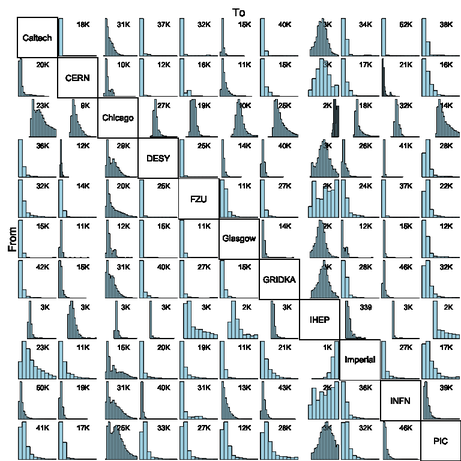
\includegraphics{full-mesh}
\caption{Transfer performance for the IPv6 testbed continuous transfers. A 1 GB file is transferred between each pair of sites, then deleted, then transferred again, continuously. The plots show the distribution of transfer duration times per site pair. The source site is named in the row, the destination site is named in the column. So the top-right plot shows transfers from Caltech to PIC, the bottom-left shows transfers fromPIC to Caltech. The x-axis is in seconds, from 0 to 500 for each plot. The number inset in each plot shows the approximate number of transfers between that site pair in that direction.}\label{fig:full-mesh}
\end{figure}

\begin{figure}[htp]
\centering
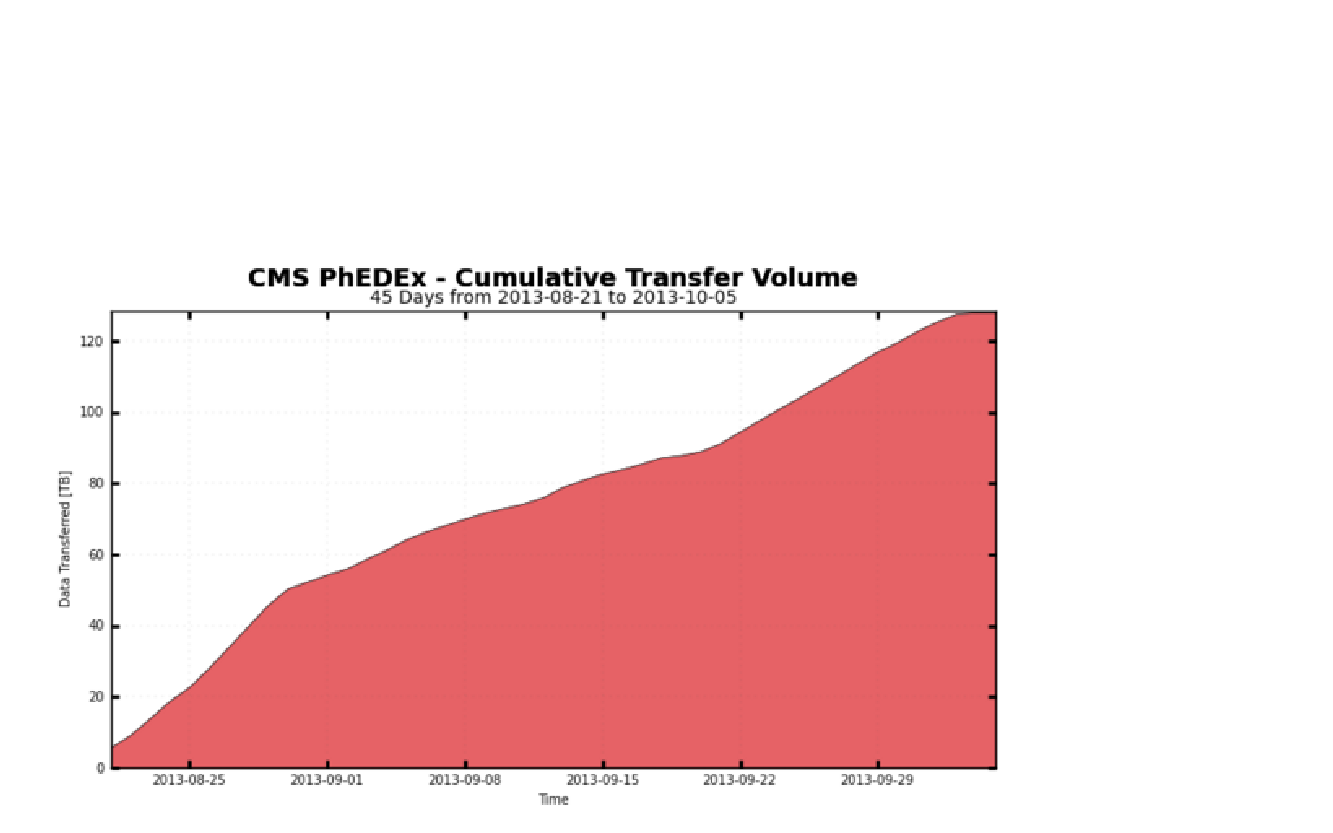
\includegraphics{phedex-transfer-volume}
\caption{Cumulative data-transfer between Imperial College and Glasgow using PhEDEx on the IPv6 testbed.}\label{fig:phedex-transfer-volume}
\end{figure}

